\documentclass[paper=letter,11pt]{scrartcl}

\KOMAoptions{headinclude=true, footinclude=false}
\KOMAoptions{DIV=14, BCOR=5mm}
\KOMAoptions{numbers=noendperiod}
\KOMAoptions{parskip=half}
\addtokomafont{disposition}{\rmfamily}
\addtokomafont{part}{\LARGE}
\addtokomafont{descriptionlabel}{\rmfamily}
%\setkomafont{pageheadfoot}{\normalsize\sffamily}
\setkomafont{pagehead}{\normalsize\rmfamily}
%\setkomafont{publishers}{\normalsize\rmfamily}
\setkomafont{caption}{\normalfont\small}
\setcapindent{0pt}
\deffootnote[1em]{1em}{1em}{\textsuperscript{\thefootnotemark}\ }


\usepackage{amsmath}
\usepackage[varg]{txfonts}
\usepackage[T1]{fontenc}
\usepackage{graphicx}
\usepackage{xcolor}
\usepackage[american]{babel}
% hyperref is needed in many places, so include it here
\usepackage{hyperref}

\usepackage{xspace}
\usepackage{multirow}
\usepackage{float}


\usepackage{braket}
\usepackage{bbm}
\usepackage{relsize}
\usepackage{tcolorbox}

\def\ketY{\ensuremath{\ket {\Psi}}}
\def\iGeV{\ensuremath{\textrm{GeV}^{-1}}}
%\def\mp{\ensuremath{m_{\textrm{proton}}}}
\def\rp{\ensuremath{r_{\textrm{proton}}}}
\def\me{\ensuremath{m_{\textrm{electron}}}}
\def\aG{\ensuremath{\alpha_G}}
\def\rAtom{\ensuremath{r_{\textrm{atom}}}}
\def\rNucl{\ensuremath{r_{\textrm{nucleus}}}}
\def\GN{\ensuremath{\textrm{G}_\textrm{N}}}
\def\ketX{\ensuremath{\ket{\vec{x}}}}
\def\ve{\ensuremath{\vec{\epsilon}}}


\def\ABCDMatrix{\ensuremath{\begin{pmatrix} A &  B  \\ C  & D \end{pmatrix}}}
\def\xyprime{\ensuremath{\begin{pmatrix} x' \\ y' \end{pmatrix}}}
\def\xyprimeT{\ensuremath{\begin{pmatrix} x' &  y' \end{pmatrix}}}
\def\xy{\ensuremath{\begin{pmatrix} x \\ y \end{pmatrix}}}
\def\xyT{\ensuremath{\begin{pmatrix} x & y \end{pmatrix}}}

\def\IMatrix{\ensuremath{\begin{pmatrix} 0 &  1  \\ -1  & 0 \end{pmatrix}}}
\def\IBoostMatrix{\ensuremath{\begin{pmatrix} 0 &  1  \\ 1  & 0 \end{pmatrix}}}
\def\JThree{\ensuremath{\begin{pmatrix}    0 & -i & 0  \\ i & 0  & 0 \\ 0 & 0 & 0 \end{pmatrix}}} 
\def\JTwo{\ensuremath{\begin{bmatrix}    0 & 0 & -i  \\ 0 & 0  & 0 \\ i & 0 & 0 \end{bmatrix}}}
\def\JOne{\ensuremath{\begin{bmatrix}    0 & 0 & 0  \\ 0 & 0  & -i \\ 0 & i & 0 \end{bmatrix}}}
\def\etamn{\ensuremath{\eta_{\mu\nu}}}
\def\Lmn{\ensuremath{\Lambda^\mu_\nu}}
\def\dmn{\ensuremath{\delta^\mu_\nu}}
\def\wmn{\ensuremath{\omega^\mu_\nu}}
\def\be{\begin{equation*}}
\def\ee{\end{equation*}}
\def\bea{\begin{eqnarray*}}
\def\eea{\end{eqnarray*}}
\def\bi{\begin{itemize}}
\def\ei{\end{itemize}}
\def\fmn{\ensuremath{F_{\mu\nu}}}
\def\fMN{\ensuremath{F^{\mu\nu}}}
\def\bc{\begin{center}}
\def\ec{\end{center}}
\def\nus{$\nu$s}

\def\adagger{\ensuremath{a_{p\sigma}^\dagger}}
\def\lineacross{\noindent\rule{\textwidth}{1pt}}

\newcommand{\multiline}[1] {
\begin{tabular} {|l}
#1
\end{tabular}
}

\newcommand{\multilineNoLine}[1] {
\begin{tabular} {l}
#1
\end{tabular}
}



\newcommand{\lineTwo}[2] {
\begin{tabular} {|l}
#1 \\
#2
\end{tabular}
}

\newcommand{\rmt}[1] {
\textrm{#1}
}


%
% Units
%
\def\m{\ensuremath{\rmt{m}}}
\def\GeV{\ensuremath{\rmt{GeV}}}
\def\pt{\ensuremath{p_\rmt{T}}}


\def\parity{\ensuremath{\mathcal{P}}}

\usepackage{cancel}
\usepackage{ mathrsfs }
\def\bigL{\ensuremath{\mathscr{L}}}

\usepackage{ dsfont }



\usepackage{fancyhdr}
\fancyhf{}


\lhead{\Large 33-444} % \hfill Introduction to Particle Physics \hfill Spring 2022}
\chead{\Large Introduction to Particle Physics} % \hfill Spring 2022}
\rhead{\Large Spring 2022} % \hfill Introduction to Particle Physics \hfill Spring 2022}

\begin{document}
\thispagestyle{fancy}

\begin{center}
{\huge \textbf{Lecture 10}}
\end{center}

{\fontsize{14}{16}\selectfont

\textbf{\underline{QFT Continued...}} 

{\Large \underline{\textbf{Summary From Last Time}}}


\begin{figure}[h]
\centering
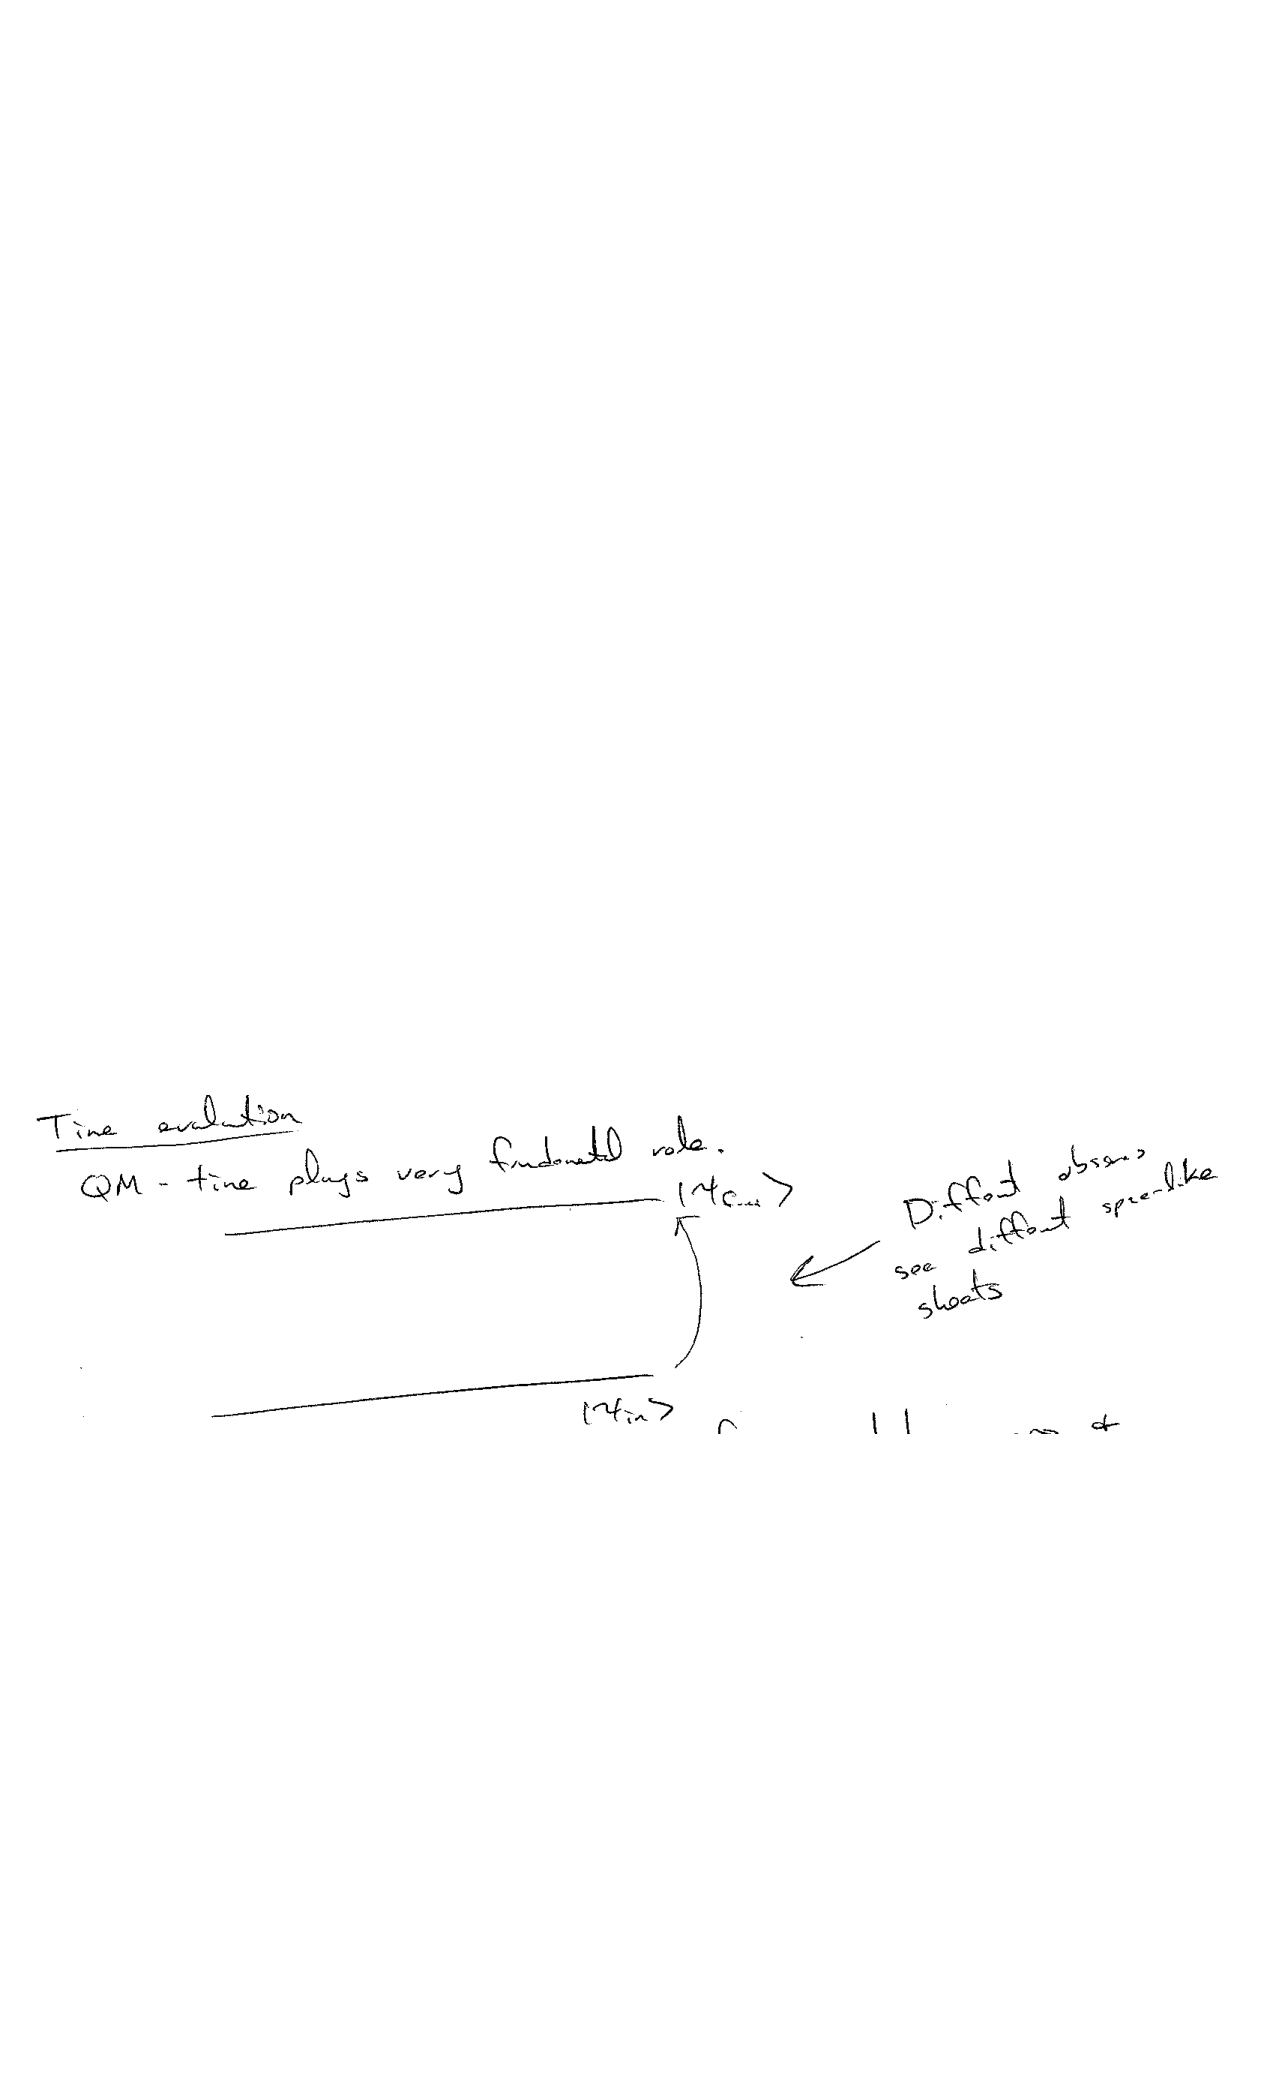
\includegraphics[width=0.9\textwidth]{./TimeEvolution.pdf}
\end{figure}

Only have a hope of Lorentz invariance if we start at -$\infty$ and go to +$\infty$.

Throw particles in from $\infty$ let them scatter \& go back out to $\infty$.

\underline{Define S-Matrix}

\be
\underbrace{\ket{p_1 \sigma_1,...p_n\sigma_n}}_{t=-\infty} \rightarrow \underbrace{\mathcal{S} \ket{p_1\sigma_1,...p_n\sigma_n}}_{t=+\infty}
\ee

$\mathcal{S}$ might be (at least a hope) Lorentz Invariant.


\noindent\rule{\textwidth}{1pt}

\textbf{Big Picture:}
The plan is to Figure out what $\mathcal{S}$ is in a totally generic theory, then see what it would take to make it Lorentz Invariant. 

Sure doesn't look like it will be L.I. 
$\mathcal{S}$ is the only object that you could even have a hope to make L.I.

We will see that for \underline{very special} choices of the interaction it will barely be possible for it to be Lorentz Invariant. 
These choices force on us anti-particle and the connection between spin and statistics. 

\noindent\rule{\textwidth}{1pt}

Something annoying that we should get rid of right away. 
Free evolution, just evolves w/phase. Totally irrelevant part.


Standard way of removing the free evolution \underline{``Interaction Representation''}.

\be
H = H_\textrm{free} + H_\textrm{Int}
\ee


\be
i \frac{d \ket{\psi}}{d t} = \left(H_\textrm{free} + H_\textrm{Int} \right) \ket{\psi} 
\ee

\underline{For $H_\textrm{Int}$ = 0}

\be
\ket{\psi} = e^{-i H_f t} \ket{\psi_{in}}
\ee

Now, we don't have a free theory, but if the interaction is small going to be pretty close to evolving like this. 


\begin{equation}\label{eq:def}
\ket{\psi} = e^{-i H_f t} \underbrace{\ket{\psi_{I}}}_{\textrm{definition}}
\end{equation}

If $H_\textrm{Int} = 0, \ket{\psi_\textrm{Int}}$ doesn't evolve at all.
Bc there is $H_\textrm{Int}$, $\ket{\psi_\textrm{Int}}$ will evolve. 

\bea
i \frac{d }{d t} \ket{\psi} &=& H_\textrm{f} \ket{\psi} + e^{-i H_f t} i \frac{d }{d t} \ket{\psi_I} \\
&=& (H_f + H_\textrm{int}) e^{-i H_f t} \ket{\psi_I}
\eea

Note: first line from derivative of~\ref{eq:def}, the second from the Schrodinger Equation.

The RHSs imply, 

\be
i \frac{d }{d t} \ket{\psi_I} =  \underbrace{e^{+i H_f t} H_\textrm{Int} e^{-i H_f t}}_{\textrm{Interaction Hamiltonian in the interaction representation}}  \ket{\psi_I} 
\ee


So, 

\be
i \frac{d }{d t} \ket{\psi_I} =  H_I  \ket{\psi_I} 
\ee
where $H_I$ can be time dependent. 

\underline{Lets formally solve this} 

Just integrating gives,

\be
\ket{\psi_I (t_2)} = \ket{\psi_I (t_1)} - i \int_{t_1}^{t_2} dt H_I \ket{\psi_I(t)}
\ee

Now we can keep iterating, 

\be
 = \ket{\psi_I (t_1)} - i \int_{t_1}^{t_2} dt H_I(t) \left( \ket{\psi_I (t_1)} - i \int_{t_1}^{t} dt' H_I(t') \ket{\psi_I(t')}\right)
\ee

or

\be
 = \ket{\psi_I (t_1)} - i \int_{t_1}^{t_2} dt H_I \ket{\psi_I (t_1)}  +  (-i)^2 \int_{t_1}^{t_2} dt \int_{t_1}^{t} dt' H_I(t)H_I(t')\ket{\psi_I(t')}
\ee

Pattern is clear,  can keep going...

\bea
\ket{\psi_I (t_2)} = [ &1& + (-i) \int_{t_1}^{t_2} dt H_I(t) \\
    &+& (-i)^2 \int_{t_1}^{t_2} dt \int_{t_1}^{t} dt' H_I(t)H_I(t') \\
    &+&  (-i)^3 \int_{t_1}^{t_2} dt \int_{t_1}^{t} dt' \int_{t}^{t'} dt'' H_I(t) H_I(t') H_I(t''') \\
    &+& ...  ] \ket{\psi_I (t_1)}
\eea

If $H_I$ is small this is giving us some nice perturbation theory. 

\begin{figure}[h]
\centering
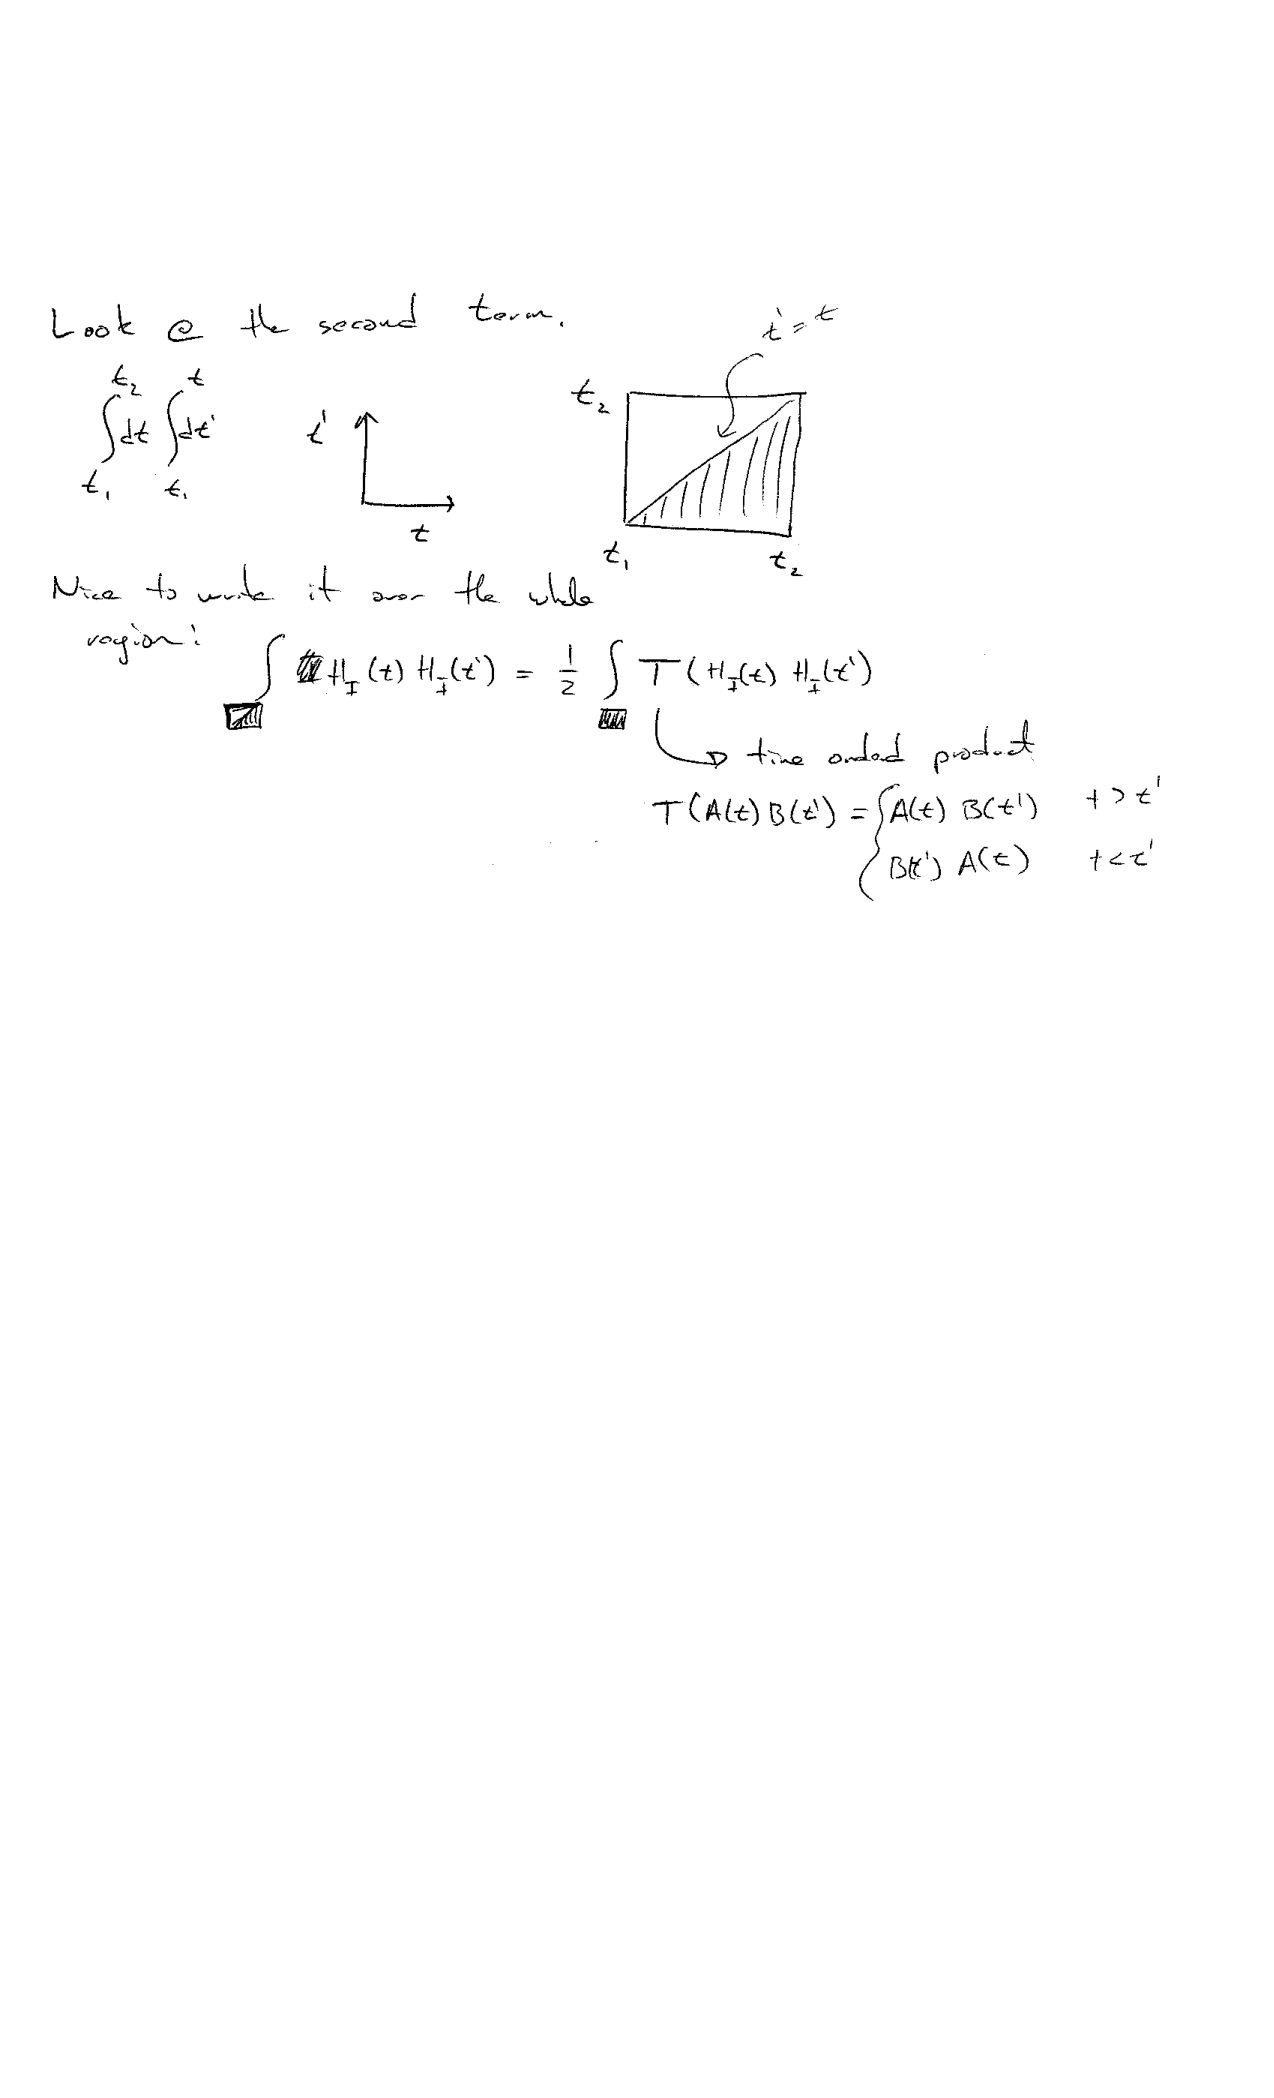
\includegraphics[width=0.9\textwidth]{./IntegrationLimits.pdf}
\end{figure}


\bea
\ket{\psi_I (t_2)} = [ &1& + (-i) \int_{t_1}^{t_2} dt \top(H_I(t)) \\
    &+& \frac{(-i)^2}{2!} \int_{t_1}^{t_2} dt \int_{t_1}^{t} dt' \top(H_I(t)H_I(t')) \\
    &+&  \frac{(-i)^3}{3!} \int_{t_1}^{t_2} dt \int_{t_1}^{t} dt' \int_{t}^{t'} dt'' \top(H_I(t) H_I(t') H_I(t''')) \\
    &+& ...  ] \ket{\psi_I (t_1)}
\eea


\be
\ket{\psi_I (t_2)} = \top\left( e^{ (-i) \int_{t_1}^{t_2} dt H_I(t)} \right)\ket{\psi_I (t_1)}
\ee

Now, let $t_1$ and $t_2$ go to $\infty$,


\be
\ket{\psi_I (+\infty)} = \top\left( e^{ (-i) \int_{-\infty}^{+\infty} dt H_I(t)} \right)\ket{\psi_I (-\infty)}
\ee

OK, Lets go back to field theory....

\noindent\rule{\textwidth}{1pt}

\be
\phi_+ (\vec{x}) = \int \cancel{d}^3p\ e^{-i \vec{p} \vec{x}}\ a^{\dagger}_{\vec{p}}
\ee

(use scalars for the moment) 

Need to build $H_I$ out of $\phi_{+/-}$ in the interaction representation.

\fbox{\begin{minipage}{\textwidth}
Note: 
\be
\phi_+^I (x, t) = e^{+iH_ft} \phi(x) e^{-iH_ft} \rightarrow e^{iE_p t} \phi(x) \\
\ee


The $e^{iHt}$ will go to $e^{-iEt}$, then $\phi(x)$ will create a new particle with energy $E_p$, and then the $e^{+iHt}$ will give $e^{+i(E+E_p) t}$

\end{minipage}}

\bea
\phi_+^I (x, t) &=& e^{+iH_ft} \phi(x) e^{-iH_ft} \\
                &=& \int \cancel{d}^3p\ e^{-i \vec{p} \vec{x}}\ e^{+iE_pt}\ a^{\dagger}_{\vec{p}} \\
                &=& \int \cancel{d}^3p\ e^{i p^\mu x_\mu}\ a^{\dagger}_{\vec{p}}
\eea

this behaves nicely under Lorentz Transforms $\phi(\Lambda x) = \phi(x)$

We seem to be in awesome shape, lets write down an interaction. 

\be
H_I = \int d^3x\ k \left[  \phi_+^I(x) ... \phi_-^I(x) \right]
\ee

and now we know how to turn this into the $\mathcal{S}$-matrix 


\be
\top\left( e^{ (-i) \int_{-\infty}^{+\infty} dt\ d^3x\ k \left[ \phi_+(x) ... \phi_-(x) \right]} \right)
\ee


\be
\top\left( e^{ (-i) \int_{-\infty}^{+\infty} d^4x\ k \left[ \phi_+(x) ... \phi_-(x) \right]} \right)
\ee

All of this is Lorentz Invariant!
Seems like we are done.

What is the problem?

Problem is the time ordering.  
Only thing that is not necessarily L.I.

This would be LI if $\top$ was LI. 
But space-like separated objects are not time-ordered in a LI way. 

Diagram: 


Only way to be LI if $H_I(x)$ and $H_I(x')$ commute when x and x' are space-like separated.

Lorentz Invariant $\Rightarrow [H_I(x), H_I(x')] = 0$  if $x-x' < 0$ (space-like). 

Now can ask if the $\phi^\dagger$'s or the $\phi$'s commute outside the light cone.  
\underline{They do Not}. 

However can find a new combination which does.

\noindent\rule{\textwidth}{1pt}

Now just state some results...

\underline{Turns out} 

\be
[\phi_+(x), \phi_+^\dagger(x')] \ne 0 \textrm{ for } x-x'<0
\ee
But we can define 

\be
\Phi(x) = \phi_+(x) + \phi_-(x) = \int \cancel{d}^3p (a^\dagger e^{-ipx} + a e^{ipx})
\ee

Can show that,
\be
[\Phi(x), \Phi(x')] = 0 \textrm{ for } x-x'<0
\ee
Only if $[a,a^\dagger] = 0$, not if $\{a,a^\dagger\} = 0$

Tells us that Scalars have to be Bosons!

Tells us that we need to build $H_I$ out of $\Phi$ (not $\phi_+$ and $\phi_-$ separately)

eg: 

\bea
H_I &=& \lambda \Phi^4(x)\\
    &=& \lambda (\phi_+(x) + \phi_-(x)) ^4\\
    &=& \lambda \left[\underbrace{\phi_+^2\phi_-^2}_{\textrm{term saw before}}^{\textrm{2 go in 2 come out}} + \underbrace{\phi_+^4 + \phi_+\phi_-^3 ...}_{\textrm{New terms}} \right] 
\eea


No charges associated with this scalar. 


Can create it or destroy it at will (eg: $\phi_+\phi_-^3$)

How do we talk about particles with conserved charge?
This will not work ! 
Only have one choice, introduce another operator.  a's and b's.

\bea
\phi^a &=& \int a^\dagger_p\ e^{-ipx} \\
\phi^b &=& \int b^\dagger_p\ e^{-ipx} \\
\eea

And construct $\Phi$ as

\bea
\Phi &=& \phi_+^a + \phi_-^b \\
     &=&\int \cancel{d}^3p (a e^{ipx} + b^\dagger e^{-ipx})
\eea


Again we have, 
\be
[\Phi(x), \Phi(x')] = 0 \textrm{ for } x-x'<0
\ee


(Note: $\Phi$ is \underline{not} Hermitian.)
But 

\be
\int d^3x\ \Phi^\dagger(x)^2 \Phi(x)^2 
\ee
is Hermitian

Expand this out and find that everything would conserve change provided that particles of type b have opposite charge to a. 

So, if you want to talk about particles that carry some well defined charge, you must have \underline{anti-particles}.

If you put this together with s=1/2, you find that they have to $\{\ \}=0$ for the Hamiltonian to vanish outside the light cone.


}
\end{document}


